\documentclass{beamer}

%\usepackage{beamerthemesplit}
\usetheme{Darmstadt}

% Text en utf8
\usepackage{ucs}
\usepackage[utf8x]{inputenc}
% Text generat automàticament en català i partició per síl·labes
\usepackage[catalan]{babel}
% Per afegir imatges
\usepackage{graphicx}

\mode<presentation>

\title{SKD: Rootkit per a sistemes operatius UNIX}
\author{Albert Sellarès Torra \\ \texttt{<whats@wekk.net>}}
\institute{Facultat d'Informàtica de Barcelona}
\date{12 de Gener de 2010}

\begin{document}

\frame{\titlepage}
% Hola bon dia,
% el meu nom és Albert Sellarès i tot seguit un presentaré el meu PFC que s'anomena
% SKD, Rootkit per a sistemes operatius UNIX.

\frame{\tableofcontents}
% Primer de tot començarem definint que és un rootkit per a tenir una idea clara de
% què és el què es vol fer.
%
% Comentaré el motiu pel qual vaig voler fer aquest projecte i quin n'era l'objectiu.
%
% Just després entrarem en detall en algunes de les funcionalitats que s'han desenvolupat
% per tal d'agafar una mica la idea de quines són les coses que es poden arribar a fer 
% amb el rootkit. 
%
% I finalment comentaré l'evolució que ha seguit el projecte, partint de la planificació 
% que es va fer durant primers dies, fins a la planificació real que ha seguit.
%
% Per acabar us mostraré les conclusions que en trec un cop realitzat.

\section{Definició}
\begin{frame}
	\frametitle{Definició de ``rootkit''}
\end{frame}

\begin{frame}
	\frametitle{Definició de ``rootkit''}
	\begin{block}{Eina o conjunt d'eines\ldots}
		\ldots que té com a finalitat ocultar-se i permetre que un tercer administri la màquina on està 
		instal·lat.
	\end{block}
\end{frame}
% El primer que hem de tenir clar, és ``què és un rootkit?''. Un rootkit és una eina o 
% conjunt d'eines que té com a finalitat ocultar-se i permetre que un tercer administri
% la màquina on està instal·lat. 

% En definitiva es pot veure com un programa en execució a la nostre màquina. 

\begin{frame}
	\frametitle{Definició de ``rootkit''}
	\begin{block}{Principals característiques:}
		\begin{itemize}
			\item S'amaga i oculta el seu funcionament.
			\item Permet l'accés al seu propietari.
			\item Permet administrar la màquina.
			\item Perdura instal·lat el màxim de temps possible.
			\item Facilita l'obtenció d'informació sensible.
		\end{itemize}
	\end{block}
	\begin{block}{Antivirus}
		Considerats com a virus per els antivirus.
	\end{block}
\end{frame}
% Tot rootkit per a poder portar a terme millor la seva tasca, ha de ocultar-se per intentar
% passar el màxim desapercebut possible. Alhora ha de permetre que el seu propietari es connecti
% a la màquina on està corrent, i l'administri (que pugui gestionar el sistema de fitxers, executar
% programes, etc).

% Cal dir que els antivirus consideren els rootkits com a un tipus de virus.

% Una característica que els rootkits comparteixen amb els virus, és la de intentar perdurar el màxim 
% de temps possible instal·lat i funcionant. Que actualitzacions del sistema o reinicis de la màquina, 
% no evitin que el rootkit deixi de ser executat.

% Finalment i com a molts virus, ens interessa que el rootkit ens ajudi a obtenir informació sensible 
% de la màquina on està instal·lat com els passwords dels usuaris o fitxers del sistema que en una 
% situació concreta ens poden permetre augmentar els nostres privilegis.

% Com es pot deduir de tot això, a ningú li agradaria tenir un rootkit en la seva màquina.

\section{Motivació}
\begin{frame}
	\frametitle{Motivació}
\end{frame}

\begin{frame}
	\frametitle{Motivació}
	\begin{block}{Motius per complicar-me la vida:}
		\begin{itemize}
			\item<1-> Passió per la seguretat informàtica.
			\item<2-> Devoció per el programari lliure i GNU/Linux.
			\item<3-> Utilitat que necessitava.
			\item<4-> Per investigar.
			\item<5-> Per aprendre.
			\item<6-> Per diversió.
%			\item<7-> $<$broma$>$Vendre'l al mercat negre i fer-me ric.$<$/broma$>$
		\end{itemize}
	\end{block}
\end{frame}
% Un cop vist què és un rootkit, anem a veure el perquè he escollit fer aquest projecte.
% El primer motiu és què estic molt posat en temes de seguretat informàtica i el tema 
% m'apassiona igual que el programari lliure en sí.
% Un altre motiu és que jo necessitava una utilitat així, es pot dir que sempre és útil
% tenir un bon rootkit sota la màniga.
% I finalment i relacionat amb els punts anteriors, per aprendre, per investigar, i en
% definitiva per diversió.

\section{Objectiu}
\begin{frame}
	\frametitle{Objectiu del projecte}
\end{frame}

\begin{frame}
	\frametitle{Objectiu del projecte}
	\begin{block}{Objectiu principal}
	Crear un rootkit multiarquitectura per a sistemes basats en UNIX que exploti al màxim 
	les característiques comentades anteriorment.
	\end{block}
\end{frame}
% Tal i com es pot haver deduït del títol, l'objectiu del projecte és justament el de crear
% un rootkit, però un rootkit multiarquitectura per a sistemes banats en UNIX que exploti 
% al màxim aquestes característiques que comentava abans que ha de tenir tot bon rootkit.
% És a dir, l'objectiu és crear un bon rootkit.

% Per a poder concretar més el nostre objectiu en el moment del plantejament del projecte,
% varem definir una sèrie de funcionalitats que creiem que havia d'oferir aquest rootkit
% per les quals varem regir tota la planificació desenvolupament i disseny.

\section{El rootkit}
\begin{frame}
    \frametitle{El rootkit}
\end{frame}

\subsection{Arquitectura}

\begin{frame}
    \frametitle{El rootkit}
	\begin{block}{El nostre rootkit:}
		\begin{itemize}
			\item \alert{Arquitectura.}
			\item Funcionalitats.
			\item Keylogger.
		\end{itemize}
	\end{block}
\end{frame}

\begin{frame}
	\frametitle{El rootkit}
	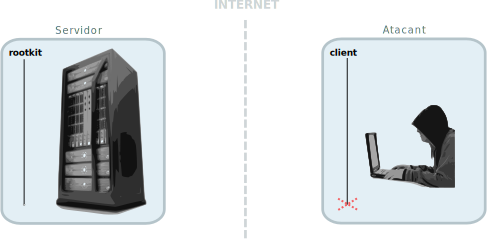
\includegraphics[scale=0.8,keepaspectratio]{arquitectura1.pdf}
\end{frame}

\begin{frame}
	\frametitle{El rootkit}
	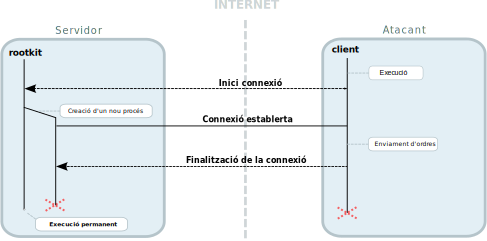
\includegraphics[scale=0.8,keepaspectratio]{arquitectura2.pdf}
\end{frame}

\begin{frame}
	\frametitle{El rootkit}
	\includegraphics[scale=0.8,keepaspectratio]{arquitectura3.pdf}
\end{frame}

\begin{frame}
	\frametitle{El rootkit}
	\includegraphics[scale=0.8,keepaspectratio]{arquitectura4.pdf}
\end{frame}

\begin{frame}
	\frametitle{El rootkit}
	\includegraphics[scale=0.8,keepaspectratio]{arquitectura5.pdf}
\end{frame}

\subsection{Funcionalitats}

\begin{frame}
    \frametitle{El rootkit}
	\begin{block}{El nostre rootkit:}
		\begin{itemize}
			\item Arquitectura.
			\item \alert{Funcionalitats.}
			\item Keylogger.
		\end{itemize}
	\end{block}
\end{frame}

\begin{frame}
	\frametitle{El rootkit}
	\begin{block}{Implementació}
		\begin{itemize}
			\item Executable sense dependències i autocontingut.
				\pause
			\item Multiarquitectura i compatible amb les variants de UNIX.
				\pause
		\end{itemize}
	\end{block}
	\begin{block}{Comunicació}
		\begin{itemize}
			\item Autenticació per contrasenya.
				\pause
			\item Comunicació xifrada.
				\pause
			\item Connexió directa.
				\pause
			\item Connexió inversa.
				\pause
			\item Protocol raw.
		\end{itemize}
	\end{block}
\end{frame}
\begin{frame}
	\frametitle{El rootkit}
	\begin{block}{Funcionalitats bàsiques}
		\begin{itemize}
			\item Tasques programades.
				\pause
			\item Heartbeat.
				\pause
			\item Ocultació.
				\pause
			\item Detecció del rootkit.
				\pause
			\item Supervivència del rootkit.
				\pause
			\item Obtenció d'una shell i un TTY.
				\pause
			\item Transferència de Fitxers.
				\pause
			\item Mode comanda / Mode servei.
		\end{itemize}
	\end{block}
\end{frame}
\begin{frame}
	\frametitle{El rootkit}
	\begin{block}{Funcionalitats avançades}
		\begin{itemize}
			\item Proxy SOCKS.
				\pause
			\item Independència de la shell.
				\pause
			\item Tècniques per evitar firewalls i filtres.
				\pause
			\item Keylogger.
		\end{itemize}
	\end{block}
\end{frame}

\subsection{Funcionalitat en detall: Keylogger}

\begin{frame}
    \frametitle{El rootkit}
	\begin{block}{El nostre rootkit:}
		\begin{itemize}
			\item Arquitectura.
			\item Funcionalitats.
			\item \alert{Keylogger.}
		\end{itemize}
	\end{block}
\end{frame}

\begin{frame}
	\frametitle{El rootkit}
	\begin{block}{Objectiu}
		Aconseguir els passwords dels diferents usuaris del sistema
	\end{block}
	\begin{block}{Característiques}
		\begin{itemize}
			\item Funcionament en entorn d'usuari.
			\item Poder capturar desde multiples serveis.
		\end{itemize}
	\end{block}
\end{frame}

\subsection*{Keylogger: Exemple de funcionament}
\begin{frame}
	\frametitle{El rootkit}
	\includegraphics[scale=0.65,keepaspectratio]{sshd_1.pdf}
\end{frame}

\begin{frame}
	\frametitle{El rootkit}
	\includegraphics[scale=0.65,keepaspectratio]{sshd_3.pdf}
\end{frame}

\begin{frame}
	\frametitle{El rootkit}
	\includegraphics[scale=0.65,keepaspectratio]{sshd_4.pdf}
\end{frame}

\begin{frame}
	\frametitle{El rootkit}
	\includegraphics[scale=0.65,keepaspectratio]{sshd_5.pdf}
\end{frame}

\begin{frame}
	\frametitle{El rootkit}
	\includegraphics[scale=0.65,keepaspectratio]{sshd_6.pdf}
\end{frame}

\begin{frame}
	\frametitle{El rootkit}
	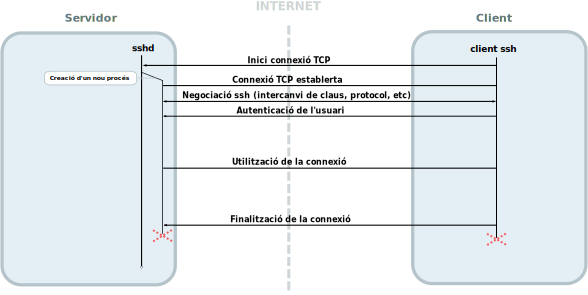
\includegraphics[scale=0.65,keepaspectratio]{sshd.pdf}
\end{frame}

\begin{frame}
	\frametitle{El rootkit}
	\includegraphics[scale=0.65,keepaspectratio]{sshd_keylogger_1.pdf}
\end{frame}

\begin{frame}
	\frametitle{El rootkit}
	\includegraphics[scale=0.65,keepaspectratio]{sshd_keylogger_2.pdf}
\end{frame}

\begin{frame}
	\frametitle{El rootkit}
	\includegraphics[scale=0.65,keepaspectratio]{sshd_keylogger_3.pdf}
\end{frame}

\begin{frame}
	\frametitle{El rootkit}
	\includegraphics[scale=0.65,keepaspectratio]{sshd_keylogger_4.pdf}
\end{frame}

\begin{frame}
	\frametitle{El rootkit}
	\includegraphics[scale=0.65,keepaspectratio]{sshd_keylogger_5.pdf}
\end{frame}

\begin{frame}
	\frametitle{El rootkit}
	\includegraphics[scale=0.65,keepaspectratio]{sshd_keylogger_6.pdf}
\end{frame}

\begin{frame}
	\frametitle{El rootkit}
	\includegraphics[scale=0.65,keepaspectratio]{sshd_keylogger_7.pdf}
\end{frame}

\begin{frame}
	\frametitle{El rootkit}
	\includegraphics[scale=0.65,keepaspectratio]{sshd_keylogger_8.pdf}
\end{frame}

\begin{frame}
	\frametitle{El rootkit}
	\includegraphics[scale=0.65,keepaspectratio]{sshd_keylogger_9.pdf}
\end{frame}

\begin{frame}
	\frametitle{El rootkit}
	\includegraphics[scale=0.65,keepaspectratio]{sshd_keylogger_10.pdf}
\end{frame}

\begin{frame}
	\frametitle{El rootkit}
	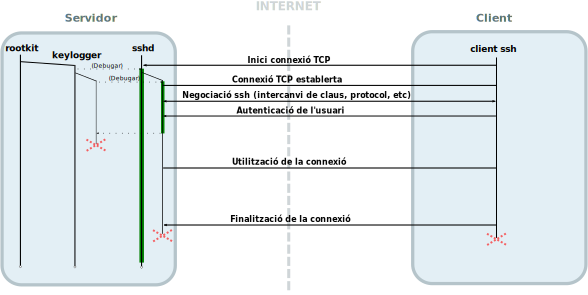
\includegraphics[scale=0.65,keepaspectratio]{sshd_keylogger.pdf}
\end{frame}

\section{Evolució}
\begin{frame}
	\frametitle{Evolució}
\end{frame}

\begin{frame}
	\frametitle{Planificació inicial}
	\hspace*{-0.38in}
	\includegraphics[scale=0.35,keepaspectratio]{gantt1.png} 
	\begin{block}{Característiques}
		\begin{itemize}
			\item No deixar la documentació pel final.
			\item Agrupació per funcionalitats.
			\item Estructura i disseny només inclou el core.
			\item Anàlisi general per conciliar-ho tot i afinar el producte.
		\end{itemize}
	\end{block}
\end{frame}

\begin{frame}
	\frametitle{Planificació final}
	\hspace*{-0.38in}
	\includegraphics[scale=0.35,keepaspectratio]{gantt2.png} 
	\begin{block}{Característiques}
		\begin{itemize}
			\item Funcionalitat de injecció no implementada.
			\item Més funcionalitats avançades a canvi.
			\item Periode d'examens i vacances no tingut en compte.
			\item Anàlisi general i conciliació ha portat molta més feina.
		\end{itemize}
	\end{block}
\end{frame}
\section{Conclusions}
\begin{frame}
	\frametitle{Conclusions}
\end{frame}

\begin{frame}
	\frametitle{Conclusions}

	\begin{block}{Motivació i objectius}
		\begin{itemize}
			\item Motivació complerta.
			\item Objectius complerts.
			\item L'única funcionalitat no complerta per motius aliens ha estat reemplaçada per altres funcionalitats.
		\end{itemize}
	\end{block}
	% He aprés i m'ho he passat bé
	% A més, donsidero que ha quedat un molt bon producte.

	\begin{block}{Part teòrica i pràctica}
		Les dues parts tenen molt de pes.
		\begin{itemize}
			\item Investigació i recerca.
			\item Prova de concepte i desenvolupament en el rootkit.
		\end{itemize}
	\end{block}
	% no només és diu el ``com'' sinó que s'implementa

	\begin{block}{Projecte amb una certa dificultat}
	Sempre és més dificil nadar contra corrent.
	\end{block}
	% Considero que aquest projecte té una certa dificultat.
	% Cal tenir en compte que darrere de 
	% SO com el GNU/Linux, hi ha molta gent que no els interessa gens que hi hagin aplicacions
	% com aquest rootkit. Grans professionals que treballen exclusivament per a 
	% fer els sistemes més segurs i per a què els processos no es puguin ocultar ni els passwords
	% ser capturats per altres usuaris.

\end{frame}

\begin{frame}
    \frametitle{Conclusions}
	\begin{block}{En definitiva\ldots}
	 \ldots es pot dir que m'he complicat una mica la vida però ha valgut la pena. :)
	\end{block}
\end{frame}
\section*{Preguntes}
\begin{frame}
    \frametitle{Preguntes?}

% Ojo amb la definició que vaig utilitzar a la memòria
% 
% ¿Cómo surgió el PFC?
% ¿Qué te parece este tema como PFC? ¿Crees suficiente como para un proyecto
% final de
% carrera? ¿Cómo has aprovechado los conocimientos de la carrera en él?
% ¿Qué partes te han costado más/menos? ¿Qué partes te han gustado más/menos?
% ¿Cuál ha sido la metodología o el proceso a realizar para completar este
% proyecto?
% ¿Por qué has elegido esta alternativa y no otra?
% Si el PFC está hecho entre varios, ¿Cómo os habéis repartido el trabajo y como
% os habéis
% sincronizado?
% ¿Por qué te pareció interesante hacer este PFC?
% ¿Se han cumplido los objetivos marcados al principio?
% 
% 
% 
% - 25 minuts
% - imprimir en paper el què he de dir en la seguent o les transpas així dono
%   temps entre transparència i transparència.
% - portar aigua
% - intentar posar cosetes de broma per trencar el gel
% - preparar-me la pregunta de l'especificació i disseny, q realment ha estat
%   més investigació (tia de LSI)

\end{frame}

\end{document}

